\documentclass[11pt,a4paper]{article}
\usepackage{amsmath,amssymb,amsthm}
\usepackage{mathtools}
\usepackage{bm}
\usepackage{booktabs}
\usepackage{array}
\usepackage{enumitem}
\usepackage{geometry}
\usepackage{graphicx}
\usepackage{subcaption}
\usepackage{xcolor}
\usepackage{tcolorbox}
\usepackage{listings}
\usepackage[pdfencoding=auto,psdextra]{hyperref}

\geometry{margin=2.5cm}
\setlength{\emergencystretch}{3em}

\newcommand{\E}{\mathbb{E}}
\newcommand{\Var}{\mathrm{Var}}
\newcommand{\R}{\mathbb{R}}
\newcommand{\norm}[1]{\left\lVert #1 \right\rVert}
\newcommand{\dt}{\Delta t}
\newcommand{\KL}{\mathrm{KL}}
\newcommand{\N}{\mathcal{N}}
\newcommand{\sgn}{\mathrm{sg}}
\newcommand{\str}{\sigma_{\mathrm{tr}}}
\newcommand{\muold}{\mu_{\mathrm{old}}}
\newcommand{\muT}{\mu_{T}}
\newcommand{\mus}{\mu_{\theta}}

\newtheorem{proposition}{Proposition}
\newtheorem*{remark*}{Remark}

\lstset{
  basicstyle=\ttfamily\small,
  breaklines=true,
  columns=fullflexible,
  keepspaces=true,
  frame=single,
  framesep=4pt,
  xleftmargin=4pt,
}

\title{\textbf{The exact latent-sum P-OPD gate switches the teacher off}\\[0.3em]
\large Why $T=1$ does not train, what causes it, and the temperature that follows}
\author{measured on probe run \texttt{w10kj2v8} (FLUX.2-klein 9B $\to$ 4B)}
\date{2026-07-30}

\begin{document}
\maketitle

\begin{abstract}
P-OPD gates teacher matching by the posterior responsibility of the teacher component in a
two-component Gaussian mixture over the observed transition. At the documented default
\texttt{popd\_temperature}$=1.0$, the responsibility is the \emph{exact} joint density ratio
summed over all latent dimensions. This note records that this setting does not train: measured
on a 9B$\to$4B probe, $75.4\%$ of transitions fall below $\gamma=0.01$, the median responsibility
is $8\times10^{-12}$, and \texttt{grad\_norm} sits at $2.2\times10^{-5}$ with a loss of
$9.9\times10^{-7}$. The cause is not a bad teacher and not a bug --- the implementation checks
out to five decimals --- but dimension aggregation: the joint KL obeys
$K=\tfrac{D}{2}w^2$ with $D=131072$, so a per-dimension mismatch of $w=0.4\%$ of one noise
standard deviation already half-closes the gate, and the measured $w$ reaches $9.8\%$. A second
observation is that $K$ varies by $1.2\times10^{4}$ along the denoising axis while varying only
$\approx\!30\%$ between samples at fixed step, so at any single global temperature the gate is
primarily a weighting along the trajectory, decomposing into $226\times$ from scheduler geometry
and $53\times$ from a genuine growth of the teacher--student velocity gap. The temperature
deployed for the long run follows from the measurement: $T=\bar{K}=107$ with $\alpha=0.731$.
\end{abstract}

\tableofcontents

%% ============================================================
\section{The gate under test}
\label{sec:setup}
%% ============================================================

Let $x_t$ be the on-policy state reached by the behavior student, and let the sampler take a
stochastic step with a model-independent scalar covariance $\str^2 I$
(\texttt{Flow-SDE}/\texttt{Dance-SDE}: $\str^2=\mathrm{std\_dev\_t}^2\,\lvert\dt\rvert$;
\texttt{CPS}: $\str^2=\mathrm{std\_dev\_t}^2$). Three transition means live at that state: the
behavior mean $\muold$ that actually produced the observed next latent $y$, the teacher mean
$\muT$, and the trainable student mean $\mus$. P-OPD forms
\begin{align}
\log\rho &= \log\frac{\N(y\mid\muT,\str^2 I)}{\N(y\mid\muold,\str^2 I)}
          = \sum_{i=1}^{D}\frac{(y_i-\muold{}_{,i})^2-(y_i-\muT{}_{,i})^2}{2\str^2},
\label{eq:logrho}\\[0.3em]
\gamma &= \sigma\!\left(\operatorname{logit}\alpha + \frac{\log\rho}{T}\right),
\qquad
\mathcal{L} = \E_{\mathrm{batch}}\!\left[\sgn(\gamma)\cdot
  \frac{1}{D}\sum_{i=1}^{D}\frac{(\mus{}_{,i}-\muT{}_{,i})^2}{2\str^2}\right],
\label{eq:gate}
\end{align}
where $D$ is the latent event dimension, $\alpha\in(0,1)$ is the prior probability of the teacher
component, $T>0$ is the temperature, and $\sgn$ is a stop-gradient. Code: \texttt{compute\_popd\_responsibility} and
\texttt{compute\_popd\_gaussian\_mean\_kl} in
\path{src/flow_factory/trainers/xopd/common.py}, wired through
\texttt{\_precompute\_popd\_step\_caches} and
\texttt{\_optimize\_train\_pass} in
\path{src/flow_factory/trainers/xopd/trainer.py}.

The quantity that will carry the whole analysis is the joint KL between the two Gaussians,
\begin{equation}
K \;=\; \KL\big(\N(\muold,\str^2 I)\,\big\|\,\N(\muT,\str^2 I)\big)
  \;=\; \frac{\norm{\muT-\muold}^2}{2\str^2},
\label{eq:K}
\end{equation}
logged per sample as \texttt{popd/teacher\_old\_kl\_joint}. Note that \eqref{eq:K} is the
dimension-summed version of the transition KL $L_{\mathrm{KL}}$ of
\texttt{per\_timestep\_loss\_dominance\_theory.tex}, with the SDE transition variance
$\str^2$ in place of the flow-matching noise fraction; that note's analysis of late-step
dominance therefore applies directly and is picked up in \S\ref{ssec:trajectory}.

%% ============================================================
\section{The exact law of the log density ratio}
\label{sec:theory}
%% ============================================================

\begin{proposition}[Gaussian law of the ratio]
\label{prop:law}
Let $y\sim\N(\muold,\str^2 I_D)$ be the observed transition, i.e.\ evaluate the ratio under the
policy that generated it. Then
\begin{equation}
\log\rho \;\sim\; \N(-K,\;2K),
\label{eq:law}
\end{equation}
and consequently $\E[\rho]=1$, $\operatorname{median}(\rho)=e^{-K}$, and
$\Pr[\rho>1]=\Phi\big(-\sqrt{K/2}\big)$.
\end{proposition}

\begin{proof}
Write $y=\muold+\str\varepsilon$ with $\varepsilon\sim\N(0,I_D)$, and let
$\Delta=\muT-\muold$. Then $y-\muT=\str\varepsilon-\Delta$ and
\begin{equation}
\norm{\str\varepsilon}^2-\norm{\str\varepsilon-\Delta}^2
  = 2\str\,\varepsilon^{\!\top}\Delta-\norm{\Delta}^2 ,
\end{equation}
so from \eqref{eq:logrho},
$\log\rho = \varepsilon^{\!\top}\Delta/\str-\norm{\Delta}^2/(2\str^2)
          = \varepsilon^{\!\top}\Delta/\str-K$.
The first term is Gaussian with mean $0$ and variance
$\norm{\Delta}^2/\str^2=2K$, which gives \eqref{eq:law}. The moment identity
$\E[\rho]=\exp(-K+\tfrac{1}{2}\cdot 2K)=1$ is the log-normal mean, as it must be since
$\E_{\pi_{\mathrm{old}}}[\rho]=\int\pi_T=1$. The median and tail probability follow from
\eqref{eq:law} directly.
\end{proof}

Two consequences shape everything below.

\paragraph{The mean of $\rho$ is uninformative.} $\E[\rho]=1$ holds for every $K$, however
large, while the median is $e^{-K}$. At the measured $K\approx100$ the median ratio is
$10^{-44}$ and the unit mean is carried entirely by excursions of probability
$\Phi(-\sqrt{K/2})=\Phi(-7.06)\approx8\times10^{-13}$. This is the familiar collapse of
importance weights in high dimension; a finite batch sees $\rho\approx0$ everywhere.

\paragraph{Saturation is a statement about $K$, not about the teacher.} At $T=1$ and
$\alpha=\tfrac12$, $\gamma<0.01$ whenever $\log\rho<-4.595$, which by \eqref{eq:law} has
probability $\Phi\big((K-4.595)/\sqrt{2K}\big)$. This exceeds $0.999$ already at $K\approx 30$.
Whether the gate is open is therefore decided by the magnitude of one scalar, and
\S\ref{sec:cause} is about what sets that magnitude.

%% ============================================================
\section{Measurement}
\label{sec:measurement}
%% ============================================================

Probe: \texttt{xopd\_configs/sde\_pathwise/flux2\_klein\_9b\_to\_4b\_popd\_diag\_t1.yaml}, three
epochs on 32 GPUs, FLUX.2-klein-base-9B teacher into a LoRA FLUX.2-klein-base-4B student,
\texttt{Flow-SDE} at \texttt{noise\_level}$=0.7$, four trained transitions per rollout drawn from
the 28-step grid, $512$px, $\alpha=0.5$, $T=1$. Run \texttt{w10kj2v8}. Because the probe performs
exactly one optimizer step per epoch, every reading below is taken at
$\theta=\theta_{\mathrm{old}}$, i.e.\ strictly on policy.

\subsection{The implementation is sound}
\label{ssec:checks}

Three logged quantities are self-validating, and they pass before any conclusion is drawn from
the run (Table~\ref{tab:checks}). This matters: a saturated gate and a broken covariance would
look alike in the loss.

\begin{table}[htbp]
\centering
\caption{Correctness checks available from the diagnostics. The first confirms that the variance
used in \eqref{eq:logrho} is the variance $y$ was actually drawn with; the second that replaying
the student on the stored state reproduces the mean the rollout used; the third that the ratio
obeys Proposition~\ref{prop:law}.}
\label{tab:checks}
\resizebox{\textwidth}{!}{%
\begin{tabular}{@{}llll@{}}
\toprule
quantity & expected & measured & verdict\\
\midrule
\texttt{popd/old\_innovation\_rms} $=\mathrm{RMS}[(y-\muold)/\str]$
  & $1$ & $0.999993\pm0.002$ & pass\\
\texttt{popd/behavior\_drift\_rms} $=\mathrm{RMS}[(\mus-\muold)/\str]$
  & $0$ at $\theta=\theta_{\mathrm{old}}$ & $0$ exactly & pass\\
$\E[\log\rho]$ vs $-K$ (Prop.~\ref{prop:law})
  & equal & $-99.60$ vs $-99.53$ ($0.07\%$) & pass\\
rollout vs replay $\str^2$, $\dt$
  & equal & no mismatch raised & pass\\
\bottomrule
\end{tabular}%
}
\end{table}

\begin{remark*}
The measured $\mathrm{sd}[\log\rho]=129.4$ is far above the $\sqrt{2K}=14.1$ that
\eqref{eq:law} predicts at fixed $K$. This is not a contradiction: the statistic pools
transitions with different $K$, and $\mathrm{sd}(K)=128.6$ across the pool. The pooled spread is
dominated by $K$ varying, not by the Gaussian draw --- the observation that
\S\ref{ssec:trajectory} turns into the main structural finding.
\end{remark*}

\subsection[At T=1 there is no training signal]
{At $T=1$ there is no training signal}
\label{ssec:dead}

\begin{table}[htbp]
\centering
\caption{Global statistics over the three probe epochs at $T=1$, $\alpha=0.5$,
$D=131072$. The gate is closed on three quarters of transitions and never opens fully; the
resulting gradient is five orders of magnitude below the clipping threshold
(\texttt{max\_grad\_norm}$=1.0$).}
\label{tab:global}
\begin{tabular}{@{}lr@{\hspace{2.2em}}lr@{}}
\toprule
quantity & value & quantity & value\\
\midrule
$\bar{K}$ (joint KL)              & $99.53$              & $\gamma$ mean          & $0.0522$\\
$\mathrm{sd}(K)$                  & $128.6$              & $\gamma$ median        & $8.4\times10^{-12}$\\
$K$ range                         & $[1.03,\,818]$       & $\gamma$ p90 / p99     & $0.196$ / $0.766$\\
$K/D$ (per dimension)             & $7.6\times10^{-4}$   & $\Pr[\gamma<0.01]$     & $0.754$\\
$\E[\log\rho]$                    & $-99.60$             & $\Pr[\gamma>0.99]$     & $0$\\
$\log\rho$ range                  & $[-803.6,\,3.66]$    & gate entropy (max $0.693$) & $0.092$\\
\midrule
\texttt{train/loss}               & $9.86\times10^{-7}$  & \texttt{train/grad\_norm} & $2.22\times10^{-5}$\\
\bottomrule
\end{tabular}
\end{table}

Figure~\ref{fig:responsibility} resolves this along the trajectory. The gate is partially open
only on the earliest steps and is off from step 16 onward, where every transition in the pool
falls below $\gamma=0.01$. The measured $\gamma$ sits slightly above the curve
$\sigma(-\bar{K}_k)$ evaluated at the mean $K$ of each step, as it must: $\gamma$ is convex in
$\log\rho$ in this regime, so averaging the gate exceeds the gate of the average.

\begin{figure}[htbp]
\centering
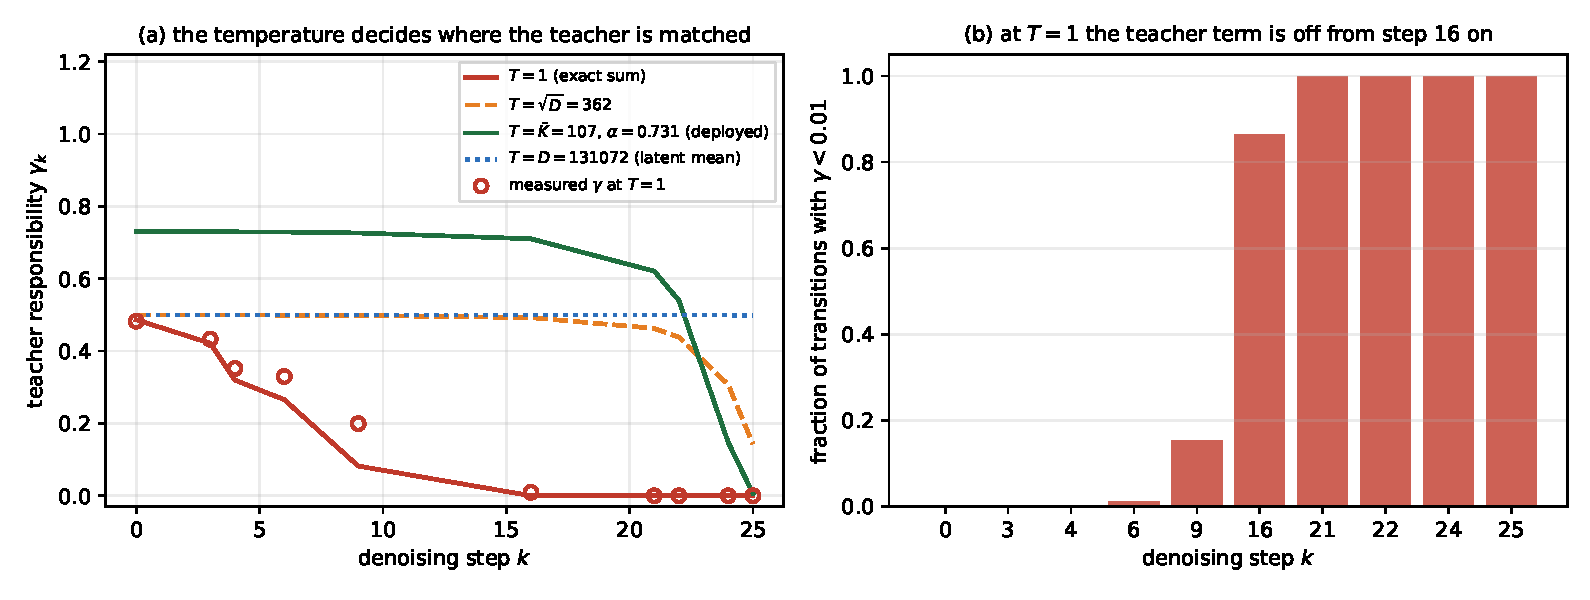
\includegraphics[width=\textwidth]{figures/popd_gate_responsibility.pdf}
\caption{(a) Teacher responsibility along the denoising axis. Curves are
$\sigma(\operatorname{logit}\alpha-\bar{K}_k/T)$ at four temperatures; circles are the probe's
measured $\gamma$ at $T=1$. $T=D$ (dotted) is flat at $\alpha$ --- a constant loss multiplier
rather than a gate. (b) Fraction of transitions with $\gamma<0.01$ at $T=1$, per step.}
\label{fig:responsibility}
\end{figure}

%% ============================================================
\section{Root cause}
\label{sec:cause}
%% ============================================================

\subsection[Dimension aggregation sets the scale of K]
{Dimension aggregation sets the scale of $K$}
\label{ssec:dimension}

Define the per-dimension mismatch in units of the transition noise,
\begin{equation}
w \;=\; \mathrm{RMS}\!\left[\frac{\muT-\muold}{\str}\right]
  \;=\; \sqrt{\frac{1}{D}\sum_{i=1}^{D}\frac{(\muT{}_{,i}-\muold{}_{,i})^2}{\str^2}} ,
\qquad\text{so}\qquad
K \;=\; \frac{D}{2}\,w^2 .
\label{eq:Kw}
\end{equation}
This is logged as \texttt{popd/teacher\_old\_gap\_whitened\_rms}, and the identity reproduces the
measured $K$ per step to within $3\%$ (Table~\ref{tab:profile}, columns $K$ and $\tfrac{D}{2}w^2$;
the residual is the difference between the mean of a square and the square of a mean).

Equation~\eqref{eq:Kw} is the root cause. An open gate at $T=1$ needs $K\lesssim1$, hence
\begin{equation}
w \;\lesssim\; \sqrt{2/D} \;=\; 3.9\times10^{-3}
\qquad\text{at}\quad D=131072 .
\label{eq:wthresh}
\end{equation}
The gate therefore demands that the teacher's transition mean agree with the student's to within
$0.4\%$ of one noise standard deviation \emph{in every one of $131072$ coordinates
simultaneously}. Two distinct models do not satisfy this except where they happen to be nearly
identical. The measured $w$ ranges from $8.9\times10^{-4}$ at step 0 --- below the threshold,
which is exactly why the gate is alive there --- to $9.8\times10^{-2}$ at step 25, a $10\%$
per-coordinate disagreement that \eqref{eq:Kw} converts into $K=648$
(Figure~\ref{fig:dimension}).

\begin{figure}[htbp]
\centering
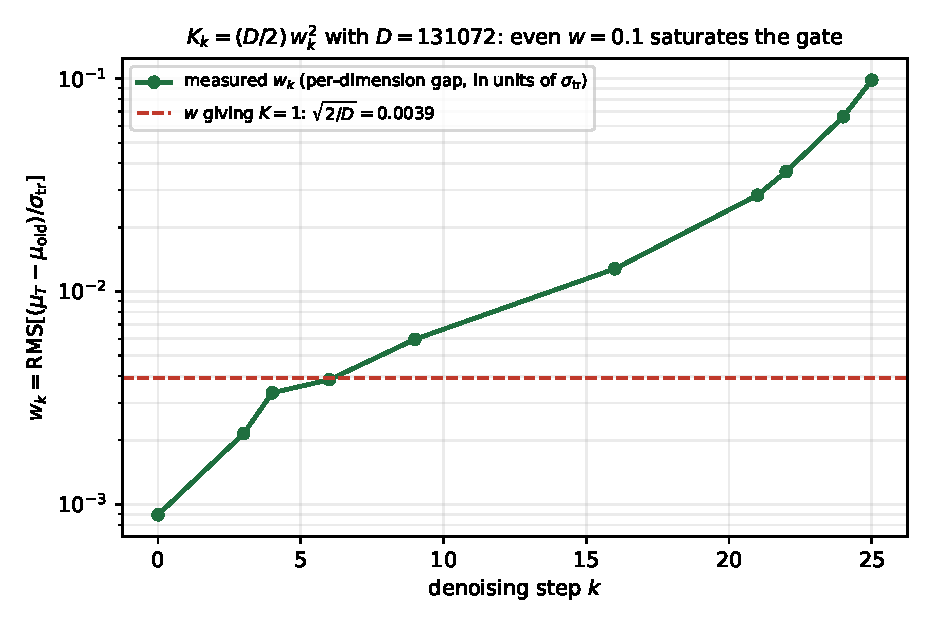
\includegraphics[width=0.72\textwidth]{figures/popd_gate_dimension.pdf}
\caption{Per-dimension mismatch $w_k$ against the threshold \eqref{eq:wthresh} at which the
exact-sum gate half-closes. The measured mismatch is small in absolute terms everywhere and
still crosses the threshold after step 4, because $K$ multiplies it by $D/2$.}
\label{fig:dimension}
\end{figure}

\begin{tcolorbox}[colback=red!4!white,colframe=red!45!black,title=Why this is not fixable by a
better teacher]
$K$ grows linearly in $D$ at fixed per-coordinate agreement. Raising the resolution from $512$px
to $1024$px multiplies $D$ by four and $K$ with it, so a gate that is marginal at one resolution
is dead at the next --- and a \emph{better} teacher only helps as $w^2$, i.e.\ halving the
per-coordinate mismatch buys a factor of four against a factor of $D$. The exact latent sum is
therefore not a tunable-but-correct choice; it is a quantity whose scale is set by the latent
dimension, which is what the temperature exists to undo.
\end{tcolorbox}

\subsection{Where along the trajectory: scheduler geometry versus a real teacher gap}
\label{ssec:trajectory}

Using $\mu=x_t+v\,\dt$ and $\str^2=\mathrm{std}^2\lvert\dt\rvert$, \eqref{eq:K} factors as
\begin{equation}
K \;=\; \frac{\norm{v_T-v_{\mathrm{old}}}^2\,\dt^2}{2\,\mathrm{std}^2\lvert\dt\rvert}
  \;=\; \underbrace{\frac{\norm{v_T-v_{\mathrm{old}}}^2}{2}}_{\text{teacher disagreement}}
        \cdot
        \underbrace{\frac{\lvert\dt\rvert}{\mathrm{std}^2}}_{\text{scheduler geometry}} .
\label{eq:Kfactor}
\end{equation}
Both factors grow toward the end of the trajectory, and the measurement separates them
(Table~\ref{tab:profile}, Figure~\ref{fig:kl}): from step 0 to step 25 the scheduler factor grows
$226\times$ (the step size grows $18\times$ while the transition variance shrinks $12\times$)
and the velocity disagreement grows $53\times$. Their product is the observed $1.2\times10^{4}$.

This is the same split that \texttt{per\_timestep\_loss\_dominance\_theory.tex} draws between
Cause~A, a parameterization artifact from $\dt^2$ amplification, and Cause~B, genuine difficulty
near the data manifold. P-OPD inherits both through $K$, and the practical consequence is
specific to the gate: at any single global $T$, the between-step variation
($1.2\times10^{4}$) overwhelms the between-sample variation at fixed step
($\mathrm{sd}(K)/K\approx0.3$, Table~\ref{tab:profile}), so
\begin{center}
\emph{one global temperature makes the responsibility a weighting along the denoising axis,\\
with only a $\pm30\%$ per-sample modulation on top.}
\end{center}
That is a weaker claim than the method's motivation suggests --- the gate is advertised as
suppressing transitions where the teacher is implausible, and it does, but under a single
temperature ``where'' is mostly ``how late in the trajectory''.

\begin{figure}[htbp]
\centering
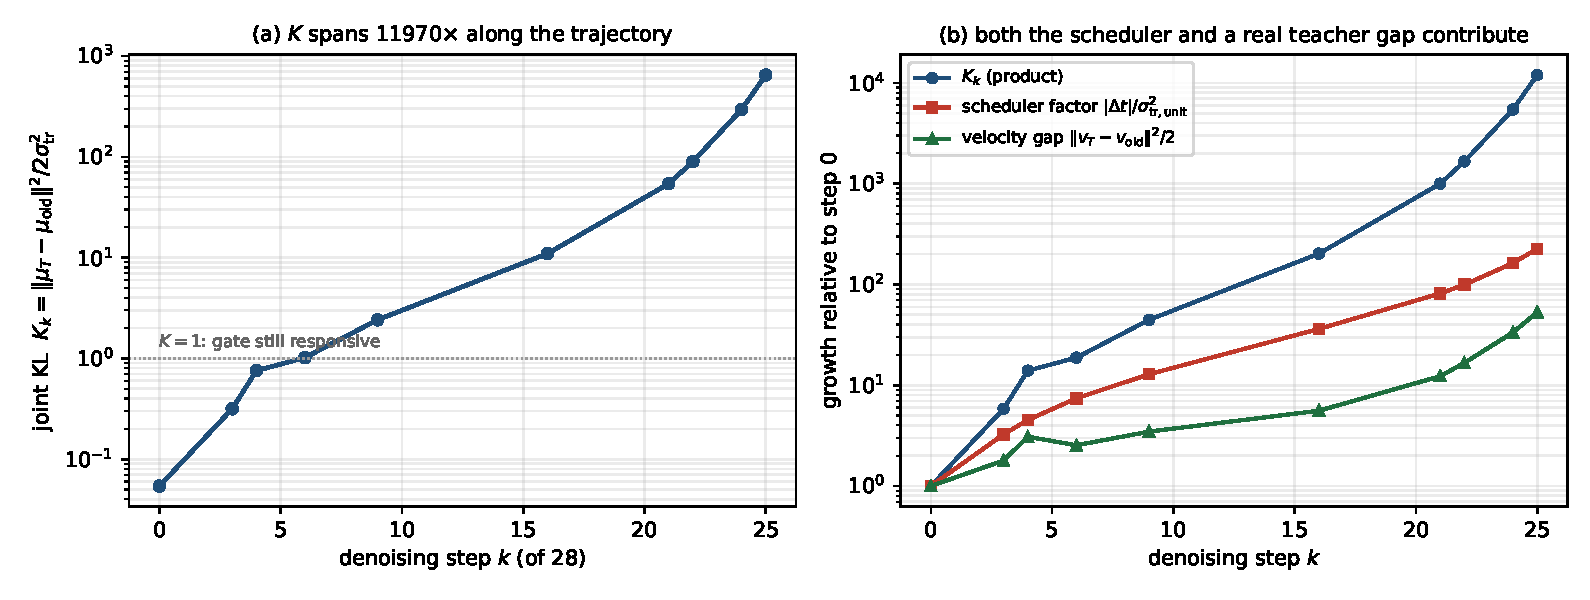
\includegraphics[width=\textwidth]{figures/popd_gate_kl_profile.pdf}
\caption{(a) Joint KL per trained step, spanning nearly four decades. (b) The factorization
\eqref{eq:Kfactor}, each curve normalized to step 0: the scheduler contributes $226\times$ and the
teacher--student velocity gap $53\times$.}
\label{fig:kl}
\end{figure}

\begin{table}[htbp]
\centering
\caption{Per-step profile from the probe (means over the pool; $D=131072$). $w$ is the
per-dimension mismatch \eqref{eq:Kw} and $\tfrac{D}{2}w^2$ its predicted $K$. The last two
columns are the measured responsibility at $T=1$ and the fraction of transitions the gate closes.
Only the ten steps drawn during the three probe epochs appear; the sampler redraws them each
epoch.}
\label{tab:profile}
\begin{tabular}{@{}rrrrrrrrr@{}}
\toprule
step $k$ & $K$ & $w$ & $\tfrac{D}{2}w^2$ & $\lvert\dt\rvert$ & $\str^2$
  & $\lvert\dt\rvert/\mathrm{std}^2$ & $\gamma$ & $\Pr[\gamma<0.01]$\\
\midrule
 0 & $0.054$ & $0.00089$ & $0.052$ & $0.0057$ & $0.490$ & $0.012$ & $0.483$ & $0.00$\\
 3 & $0.316$ & $0.00215$ & $0.304$ & $0.0070$ & $0.182$ & $0.038$ & $0.433$ & $0.00$\\
 4 & $0.755$ & $0.00334$ & $0.733$ & $0.0075$ & $0.141$ & $0.053$ & $0.352$ & $0.00$\\
 6 & $1.017$ & $0.00385$ & $0.972$ & $0.0086$ & $0.099$ & $0.087$ & $0.330$ & $0.01$\\
 9 & $2.415$ & $0.00597$ & $2.333$ & $0.0109$ & $0.073$ & $0.151$ & $0.199$ & $0.15$\\
16 & $10.95$ & $0.01278$ & $10.71$ & $0.0221$ & $0.052$ & $0.424$ & $0.009$ & $0.86$\\
21 & $54.16$ & $0.02837$ & $52.75$ & $0.0450$ & $0.047$ & $0.954$ & $0.000$ & $1.00$\\
22 & $89.93$ & $0.03656$ & $87.60$ & $0.0539$ & $0.046$ & $1.166$ & $0.000$ & $1.00$\\
24 & $294.8$ & $0.06620$ & $287.2$ & $0.0818$ & $0.043$ & $1.908$ & $0.000$ & $1.00$\\
25 & $648.0$ & $0.09838$ & $634.3$ & $0.1046$ & $0.040$ & $2.650$ & $0.000$ & $1.00$\\
\bottomrule
\end{tabular}
\end{table}

%% ============================================================
\section{Consequence: choosing the temperature}
\label{sec:temperature}
%% ============================================================

The temperature rescales $\log\rho$ before the sigmoid, so it selects which regime of
Figure~\ref{fig:responsibility} the run lives in. Table~\ref{tab:temperature} evaluates the four
candidates using the measured $K$, and Figure~\ref{fig:weight} shows the loss weight
$\gamma_k K_k$ each step ends up receiving --- the quantity that decides what the run actually
optimizes.

\begin{table}[htbp]
\centering
\caption{Temperature candidates evaluated at the measured $\bar{K}=99.5$ with
$\mathrm{sd}(K)=128.6$ and $D=131072$. Quantiles of $\gamma$ combine the Gaussian draw of
\eqref{eq:law} with the spread of $K$ across the pool. The last two columns describe the loss
weight profile over the ten observed steps.}
\label{tab:temperature}
\resizebox{\textwidth}{!}{%
\begin{tabular}{@{}llrrrrr@{}}
\toprule
setting & $T$ & $\alpha$ & $\gamma$ p01 / p50 / p99 (model) & final-step share & weight spread\\
\midrule
exact latent sum & $1$ & $0.5$ & $0.000$ / $0.000$ / $1.000$ & --- (no signal) & $10^{23}\times$\\
$\sqrt{D}$ & $362$ & $0.5$ & $0.218$ / $0.427$ / $0.665$ & $36.3\%$ & $3.4\times10^{3}\times$\\
\textbf{calibrated} & $\bm{107}$ & $\bm{0.731}$ & $0.035$ / $0.500$ / $0.965$ & $2.9\%$
  & $1.2\times10^{3}\times$\\
latent mean & $131072$ & $0.5$ & $0.499$ / $0.500$ / $0.501$ & $58.7\%$ & $1.2\times10^{4}\times$\\
\midrule
no gate ($\gamma\equiv\alpha$) & --- & $0.5$ & constant & $58.8\%$ & $1.2\times10^{4}\times$\\
\bottomrule
\end{tabular}%
}
\end{table}

The quantile column treats the pooled $\log\rho$ as one Gaussian with the measured $\bar{K}$ and
$\mathrm{sd}(K)$, so it overstates the tails: the pool is a mixture over steps whose $K$ differs by
four decades, not a single Gaussian. At $T=1$ the model gives p50/p99 of $0.000$/$1.000$ against
the measured $8\times10^{-12}$/$0.766$. It is quoted because it makes the three regimes comparable
at a glance; the exact statements are the per-step curves of Figure~\ref{fig:responsibility} and
the weight shares of Figure~\ref{fig:weight}, which use the measured per-step $K$ without this
approximation.

Read the two ends against the middle:
\begin{itemize}[leftmargin=1.4em,itemsep=0.25em]
\item $T=1$ gives no signal, for the reason of \S\ref{ssec:dimension}.
\item $T=D$ reproduces a per-dimension (latent-mean) log ratio. It is perfectly stable and
      perfectly uninformative: $\gamma$ spans $0.499$ to $0.501$, so the run is the ungated
      objective scaled by $\alpha$ --- its loss weight profile is indistinguishable from no gate
      at all ($58.7\%$ versus $58.8\%$ of the weight on the final step).
\item $T=\bar{K}$ places the median gate logit one unit below $\operatorname{logit}\alpha$;
      choosing $\alpha=\sigma(1)=0.731$ then centers the median responsibility at $0.5$, which is
      the widest usable range. Transitions closer than typical to the teacher get
      $\gamma>0.5$, further ones $\gamma<0.5$.
\end{itemize}

The deployed configuration is therefore $T=107$ (the mean $K$ over the probe's three epochs; the
final-epoch summary alone gives $99.5$) and $\alpha=0.731$, in
\path{xopd_configs/sde_pathwise/flux2_klein_9b_to_4b_popd_mix_1kep.yaml}. Its effect on
what gets optimized is substantial (Figure~\ref{fig:weight}b): the ungated objective spends
$58.8\%$ of its teacher-matching weight on the single final step, while the calibrated gate spends
$2.9\%$ there and redistributes onto steps 21--24, which is the region where the teacher is still
plausible under the student's own transition density but the two models genuinely differ.

\begin{figure}[htbp]
\centering
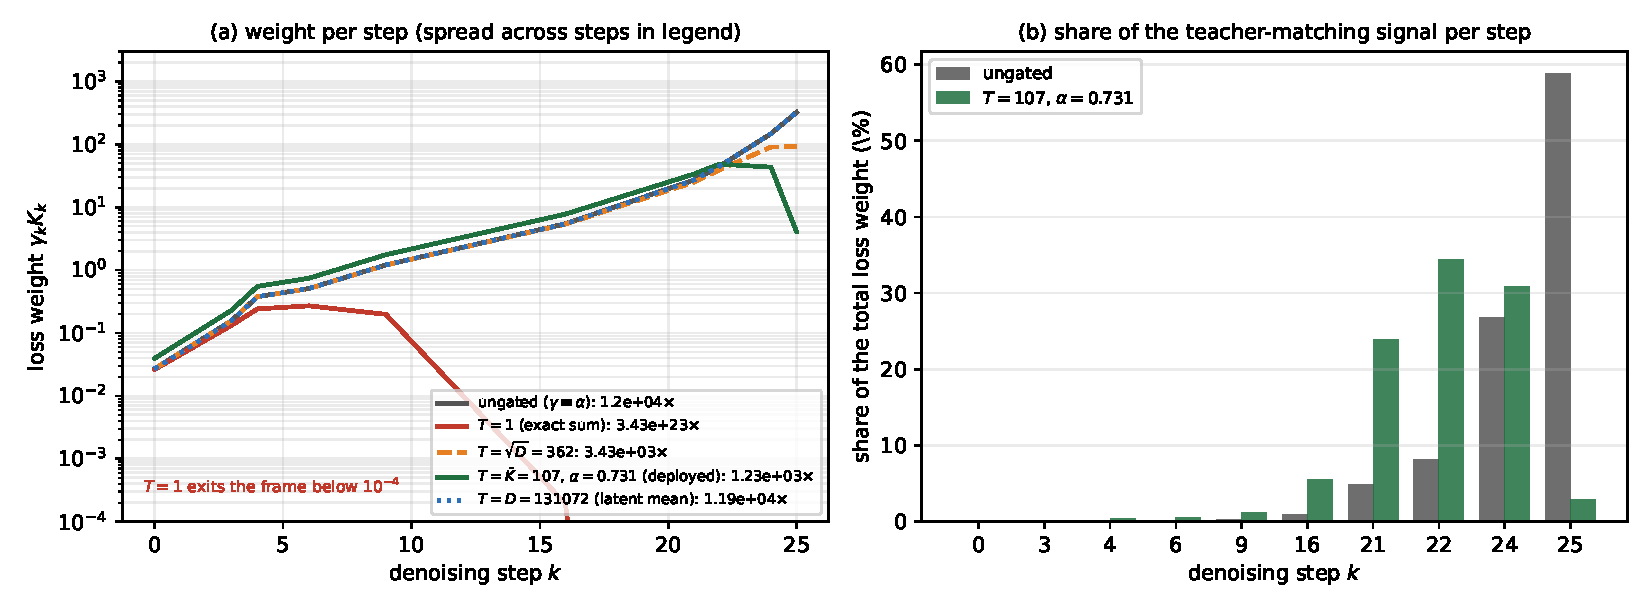
\includegraphics[width=\textwidth]{figures/popd_gate_loss_weight.pdf}
\caption{(a) Loss weight $\gamma_k K_k$ per step; the $T=1$ curve leaves the frame below
$10^{-4}$. (b) Share of the total teacher-matching weight per step, ungated versus the deployed
gate. Shares are conditional on the ten steps the probe happened to draw.}
\label{fig:weight}
\end{figure}

%% ============================================================
\section{Open points}
\label{sec:open}
%% ============================================================

\paragraph{A per-timestep temperature would make the gate per-sample.} The structural finding of
\S\ref{ssec:trajectory} is that a global $T$ spends its dynamic range on the trajectory axis.
Setting $T_k\propto\E[K_k]$ --- one temperature per denoising step, estimated online --- would
divide out the $226\times$ scheduler component and the $53\times$ systematic teacher trend,
leaving the $\pm30\%$ between-sample variation as the only driver. The gate would then mean what
the method says it means: this transition is less plausible than others \emph{at the same point
in the trajectory}. This is not implemented; it is the natural next variant if the global-$T$ arm
shows the gate doing little.

\paragraph{The gate should open as distillation proceeds.} Every number here is measured at
$\theta=\theta_{\mathrm{old}}$ with an undistilled student, so $w$ is the base 4B-versus-9B
mismatch. As training reduces $w$, $K$ falls quadratically and $\gamma$ rises, so at fixed $T$ the
gate self-anneals toward $\alpha$. \texttt{popd/gamma\_mean} and
\texttt{popd/teacher\_old\_kl\_joint} over the long run test this directly; if they do not move,
the gate is not tracking distillation progress.

\paragraph{Attribution still needs a control.} The P-OPD arm differs from the 32B$\to$4B ODE mix
baseline in the sampler, the loss space and the gate at once. Crediting any change to the gate
requires a \texttt{xopd\_target\_mode: direct} run on the identical \texttt{Flow-SDE} sampler,
which has not been run.

%% ============================================================
\section*{Reproducing}
\addcontentsline{toc}{section}{Reproducing}
%% ============================================================

\begin{lstlisting}[language=bash]
# probe (three epochs, 32 GPUs) -- the exact-sum case under test
MASTER_PORT=29620 bash scripts/xopd_cluster/run_4node_xopd.sh \
  xopd_configs/sde_pathwise/flux2_klein_9b_to_4b_popd_diag_t1.yaml

# temperature/alpha recommendation + the trajectory profile, from the probe run
python scripts/xopd_analysis/calibrate_popd_gate.py \
  --run-name flux2klein_9b_to_4b_popd_DIAG_sum_t1

# figures and the cached statistics used in this note
python scripts/xopd_analysis/plot_popd_gate_temperature.py \
  --run 315229706-xi-an-jiaotong-university-/Flow-Factory-XOPD/w10kj2v8
\end{lstlisting}

Cached probe statistics:
\path{docs/xopd/core/p_opd/figures/popd_gate_probe_stats.json}.
Algorithm reference: \path{docs/opd/cross_opd_xopd.md}, section ``P-OPD ---
probability-mixture proximal target''. Companion theory on per-step weighting:
\path{docs/xopd/core/shared/per_timestep_loss_dominance_theory.tex}.

\end{document}
